\documentclass[a4paper]{article}
\usepackage[spanish]{babel}
\usepackage[utf8]{inputenc}
\usepackage{charter}   % tipografia
\usepackage{graphicx}
\usepackage{courier}
%\usepackage{makeidx}
\usepackage{paralist} %itemize inline
\usepackage{caption}
%\usepackage{float}
%\usepackage{amsmath, amsthm, amssymb}
%\usepackage{amsfonts}
%\usepackage{sectsty}
%\usepackage{charter}
%\usepackage{wrapfig}
%\usepackage{listings}
%\lstset{language=C}
\usepackage{booktabs}

\usepackage{color} % para snipets de codigo coloreados
\usepackage{fancybox}  % para el sbox de los snipets de codigo

\definecolor{litegrey}{gray}{0.94}

% \newenvironment{sidebar}{%
% 	\begin{Sbox}\begin{minipage}{.85\textwidth}}%
% 	{\end{minipage}\end{Sbox}%
% 		\begin{center}\setlength{\fboxsep}{6pt}%
% 		\shadowbox{\TheSbox}\end{center}}
% \newenvironment{warning}{%
% 	\begin{Sbox}\begin{minipage}{.85\textwidth}\sffamily\lite\small\RaggedRight}%
% 	{\end{minipage}\end{Sbox}%
% 		\begin{center}\setlength{\fboxsep}{6pt}%
% 		\colorbox{litegrey}{\TheSbox}\end{center}}

\newenvironment{codesnippet}{%
	\begin{Sbox}\begin{minipage}{\textwidth}\sffamily\small}%
	{\end{minipage}\end{Sbox}%
		\begin{center}%
		\vspace{-0.4cm}\colorbox{litegrey}{\TheSbox}\end{center}\vspace{0.3cm}}



\usepackage{fancyhdr}
\pagestyle{fancy}

%\renewcommand{\chaptermark}[1]{\markboth{#1}{}}
\renewcommand{\sectionmark}[1]{\markright{\thesection\ - #1}}

\fancyhf{}

\fancyhead[LO]{Sección \rightmark} % \thesection\ 
\fancyfoot[LO]{\small{Nombre Apellido, Nombre Apellido, Nombre Apellido}}
\fancyfoot[RO]{\thepage}
\renewcommand{\headrulewidth}{0.5pt}
\renewcommand{\footrulewidth}{0.5pt}
\setlength{\hoffset}{-0.8in}
\setlength{\textwidth}{16cm}
%\setlength{\hoffset}{-1.1cm}
%\setlength{\textwidth}{16cm}
\setlength{\headsep}{0.5cm}
\setlength{\textheight}{25cm}
\setlength{\voffset}{-0.7in}
\setlength{\headwidth}{\textwidth}
\setlength{\headheight}{13.1pt}

\renewcommand{\baselinestretch}{1.1}  % line spacing


% \setcounter{secnumdepth}{2}
\usepackage{underscore}
\usepackage{caratula}
\usepackage{url}

%hola
% ******************************************************** %
%              TEMPLATE DE INFORME ORGA2 v0.1              %
% ******************************************************** %
% ******************************************************** %
%                                                          %
% ALGUNOS PAQUETES REQUERIDOS (EN UBUNTU):                 %
% ========================================
%                                                          %
% texlive-latex-base                                       %
% texlive-latex-recommended                                %
% texlive-fonts-recommended                                %
% texlive-latex-extra?                                     %
% texlive-lang-spanish (en ubuntu 13.10)                   %
% ******************************************************** %



\begin{document}


\thispagestyle{empty}
\materia{Organización del Computador II}
\submateria{Segundo Cuatrimestre de 2014}
\titulo{Trabajo Práctico II}
\subtitulo{SIMD}
\integrante{Christian Chibana}{586/13}{christian.chiba93@gmail.com}
\integrante{Javier Minces Müller}{231/13}{javijavi1994@hotmail.com}
\integrante{Nicolás Roulet}{587/13}{nicoroulet@gmail.com}

\maketitle
\newpage

\thispagestyle{empty}
\vfill
\begin{abstract}
En este Trabajo Práctico se implementaron cuatro filtros de imagen en dos versiones: una en lenguaje C, y una en ASM haciendo uso de las instrucciones SSE, para realizar un análisis de la performance del procesador al utilizar el modelo de programación SIMD (Single Instruction Multiple Data). 

\end{abstract}

\thispagestyle{empty}
\vspace{3cm}
\tableofcontents
\newpage


%\normalsize
\newpage

\section{Introducción}
El objetivo principal de este trabajo práctico es explorar el modelo de programación SIMD (Single Instruction Multiple Data) y realizar un análisis riguroso de los resultados de performance del procesador al hacer uso de las intrucciones SSE. Para esto, se implementaron cuatro filtros en dos versiones: una en lenguaje C, y una en ASM haciendo uso de las instrucciones SSE.

Los filtros a aplicar son los siguientes:
\begin{itemize}
\item Cropflip: recorta una imagen y la voltea verticalmente, según cuatro parámetros que indican la fracción rectangular de la imagen que se conserva: $tamx$ y $tamy$ indican las dimensiones de la porción a recortar, $offsetx$ y $offsety$ la distancia a los bordes izquierdo y superior a partir de la cual se tomará la imagen.
\begin{equation}\label{eqn:cropflip}
\textbf{dst}_{(i,j)}=\textbf{src}_{(tamy + offsety - i - 1, offsetx + j)}.
\end{equation}

\item Sierpinski: oscurece los puntos de la imagen, generando una forma similar a un triángulo de sierpinski
\begin{equation}\label{eqn:sierpinski}
\textbf{dst}_{(i,j)}=\textbf{src}_{(i,j)}*\textbf{coef}_{(i,j)}.
\end{equation}
\begin{equation}
\textbf{coef}_{(i,j)}= \frac{1}{255,0}\left (\left \lfloor{\frac{i}{cant_{filas}}*255,0}\right \rfloor \oplus \left \lfloor{\frac{j}{cant_{cols}}*255,0}\right \rfloor \right) 
\end{equation}

\item Bandas: convierte la imagen a varios tonos de gris, tomando como referencia la suma de los diferentes componentes ($r,g,b$) de cada píxel de la imagen fuente para asignar un tono de gris al píxel correspondiente de la imagen destino.

\item Motion blur: aplica un filtro de desenfoque en movimiento, aplicando a cada píxel un promedio de algunos píxeles cercanos
\begin{equation}\label{eqn:mblur}
\textbf{dst}_{(i,j)}=0.2*\textbf{src}_{(i-2,j-2)}+0.2*\textbf{src}_{(i-1,j-1)}+0.2*\textbf{src}_{(i,j)}+0.2*\textbf{src}_{(i+1,j+1)}+0.2*\textbf{src}_{(i+2,j+2)}.
\end{equation}


\end{itemize}

Para aplicar los filtros se tomó a las imágenes como una matriz de píxeles, donde cada píxel contenía 4 bytes, indicando cada uno el valor de rojo ($r$), verde ($g$), azul ($b$) y transparencia ($\alpha$). En ASM las matrices se pueden considerar como un vector, accediendo, por ejemplo, a la posición ($i, j$) mediante la posición de memoria $[A+F*i+j]$, donde $F$ es el tamaño de la fila y $A$ la posición de memoria donde se inicia la matriz.

Los filtros son aplicables tanto a imágenes como a videos. Puede verse que el ancho de las imágenes debe ser múltiplo de la cantidad de píxeles que procesamos en una iteración. %y le pusimos 250 al cropflip :D

Se comparó la performance de la versión en ASM con las versiones en C generadas con las distintas optimizaciones posibles (-O0, -O1, -O2, -O3). Esta comparación se hizo en base a los ciclos de clock que tardaba cada una en aplicar el filtro a la imagen. Para obtener la cantidad de ciclos insumidos en las versiones ASM se recurrió a la instrucción \texttt{rdtsc} (Read Time Stamp Conter), que devuelve el valor del registro TSC que se incrementa en 1 en cada ciclo de clock, comparando su valor antes de procesar el primer píxel con su valor luego de finalizar el filtro. 

Para realizar las mediciones, se utilizó siempre una computadora con procesador $i5$ de los laboratorios de computación del DC, a excepción de las mediciones del experimento \textbf{2.1.2} que consiste en correr los filtros en simultáneo con otros programas, en cuyo caso es necesario tener control sobre el \textit{power management} del procesador para establecer una frecuencia fija de clock de forma que no se distorsionen los resultados por un aumento de la frecuencia de clock producto de la cantidad de procesos corriendo en simultáneo.

\section{Desarrollo}

\subsection{Filtro cropflip}
En la implementación del filtro cropflip, se procesan 4 píxeles por iteración. No es necesario realizar ningún cálculo con los valores de $r,g,b$ de cada píxel, solamente se efectuan movimientos entre posiciones de memoria. Las operaciones realizadas en cada ciclo son las siguientes:
\begin{itemize}
\item En primer lugar se ubica la posición de memoria donde se encuentran los píxeles de la imagen fuente que se van a copiar. Basándose en la fórmula expuesta previamente, la posición de memoria a la que se quiere acceder es \texttt{[src + (tamy + offsety - i - 1) * src_row_size + (offsetx + j) * 4]} donde \texttt{src} apunta al comienzo de la matriz \textbf{src} y \texttt{src_row_size} es el ancho en memoria de cada fila de la matriz.
\item Una vez obtenida la dirección, se carga la double quadword indicada en un registro xmm. Este ahora contiene el píxel buscado y los tres siguientes.
\item Se ubica la posición donde se quiere copiar el dato en la matriz \textbf{dst}, que es \texttt{[dst + i * dst_row_size + j * 4]}.
\item Se copia el dato cargado en la posición de destino.
\end{itemize}

\subsubsection{Código generado y Optimizaciones}

Al compilar el programa \texttt{cropflip_c.c} y analizar el código assembler generado, lo primero que se observa es que la función compilada no es la única presente. Por un lado, el flag \texttt{-g} añade al código varias funciones que contienen información útil para el debugger, cuya dimensión es bastante mayor que el programa en sí. Se genera también una seccion de \texttt{rodata} con constantes utilizadas por el programa.

Asimismo, es evidente que la compilación sin optimización utiliza variables locales en la pila para almacenar datos. Ésto genera una gran cantidad de accesos prescindibles a memoria, que podrían ser minimizados con un uso más eficiente de los registros.

El compilador \texttt{cc}/\texttt{gcc} provee los siguientes flags de optimizacion: \texttt{-O0} (sin optimización), \texttt{-O1, -O2, -O3} (máxima optimización), \texttt{-Os} (\texttt{-O2} con reducción de tamaño del código generado), \texttt{-Ofast} (\texttt{-O3} más flags adicionales, no respeta estándares de compilación estrictos) y \texttt{-Og} (optimización que no interfiere con el proceso de $debugging$).

Al compilar utilizando flags de optimización es notorio desde el primer nivel que el uso de variables locales en la pila se ve reemplazado por un mayor empleo de registros para reducir los accesos a memoria, fenómeno que se acentúa en mayores niveles de optimización con el uso de flags como \texttt{-fmerge-constants}.

Por último, utilizando el flag \texttt{-O3} de optimización se observa que el programa generado hace uso de los registros xmm aprovechando las operaciones SIMD (en particular, utiliza la instrucción \texttt{movdqu} para mover múltiples píxeles en una sola iteración). Ésto se debe a que el compilador está diseñado para vectorizar ciclos sobre ciertas estructuras (flags \texttt{-ftree-vectorize, -ftree-loop-vectorize}) e incluso aplicar SIMD con diferentes niveles de profundidad (configurables con \texttt{-fsimd-cost-model}) en casos donde la operación a vectorizar sea relativamente simple, como es el caso del ciclo de cropflip.

\subsubsection{Experimentación de calidad de mediciónes}

Para medir se tomaron los siguientes parámetros:

\begin{tabular}{l|r} %cropflip
 tamx & 150 \\
 tamy & 150 \\
 offsetx & 250 \\
 offsety & 300 \\
\end{tabular}

\smallskip

Este filtro sólo recorre tantos píxeles como haya en la imagen de destino, por lo que es necesario que ésta sea lo suficientemente grande para obtener resultados confiables.

En primer lugar medimos diez veces los ciclos de clock que tardaba en ejecutarse el programa, y tomamos el promedio y la varianza. Luego, repetimos la medición mientras en cuatro terminales corríamos un programa que incrementaba en 1 una variable infinitamente. Obtuvimos los resultados mostrados en la Figura 1.

\begin{figure}[htbp]
\centering
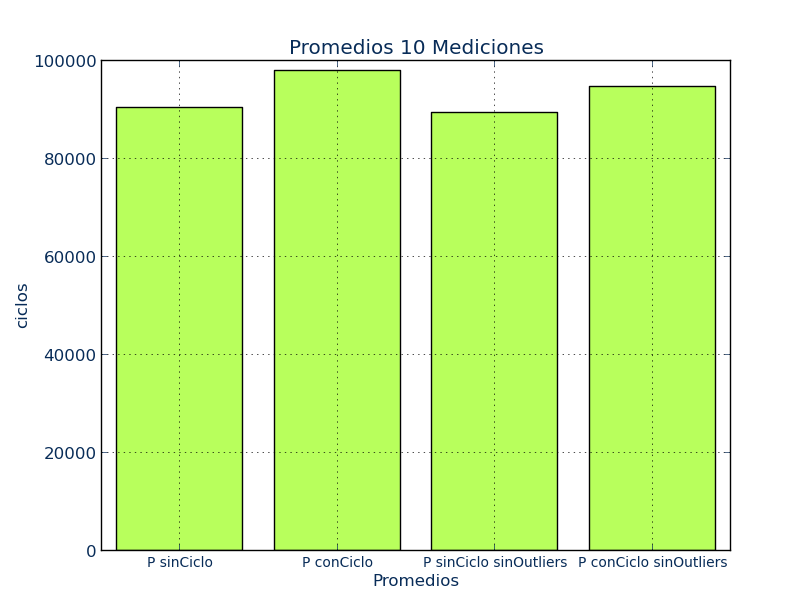
\includegraphics[scale=0.33]{imagenes/promediosFosqui.png}
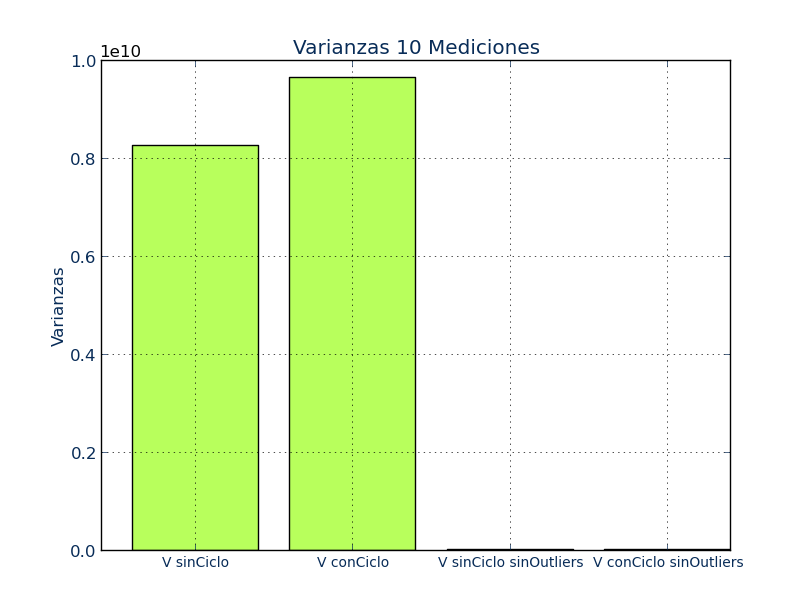
\includegraphics[scale=0.33]{imagenes/varianzaFosqui.png}
\caption{Cropflip: promedio y varianza 10 mediciones} 
\label{fig:grafico_esp-var_cropflip}
\end{figure}

Como se ve en el gráfico de promedios, al ejecutar el ciclo infinito que suma uno, aumenta la cantidad de ciclos en la ejecución del programa. En el gráfico de varianza, se puede observar que eliminando los $outliers$ se reduce considerablemente la varianza; es decir que los valores son más cercanos al promedio. 

Para obtener una mejor calidad en la experimentación y que los resultados puedan ser replicados, en los próximos experimentos se harán 100 mediciones. En cada instancia donde se compara el tiempo de ejecución de C con el tiempo de ejecución en ASM se presentan en gráficos separados los resultados ejecutando 10 y 100 mediciones. De esta forma se puede ver si hay una diferencia apreciable en la dispersión de los resultados. 

Una ejecución del programa en un entorno ideal tardaría siempre la misma cantidad de ciclos. Por lo tanto, se podría considerar outliers únicamente a los mayores valores, ya que esto indicaría que hay procesos externos que demoran la ejecución; en cambio, los menores se acercan al valor real. Sin embargo, decidimos atenernos al enunciado y descartar los 20 valores superiores e inferiores.

\subsubsection{Experimentación con optimizaciones}

Al comparar la versión en assembler con la versión en C con las distintas optimizaciones, se obtuvieron estos resultados: (ver Figura ~\ref{fig:graficos_cropflip})

\begin{figure}[htbp]
\centering
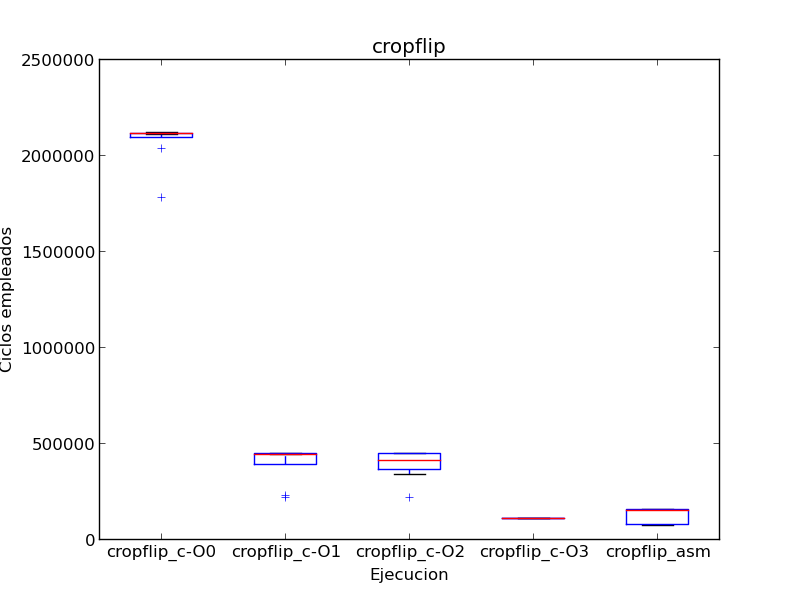
\includegraphics[scale=0.33]{imagenes/tiemposcropflip.png}
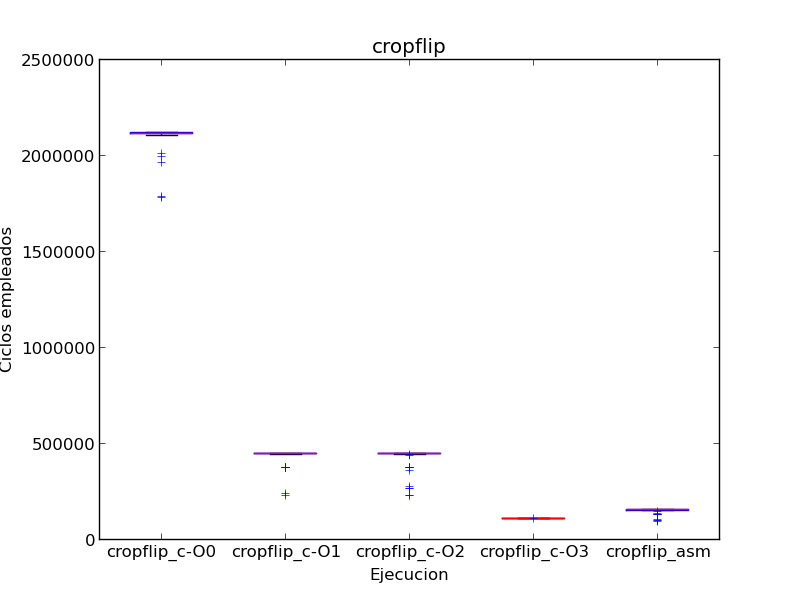
\includegraphics[scale=0.33]{imagenes/tiemposcropflip100.png}
\caption{Cropflip: 10 mediciones (izquierda) vs. 100 (derecha)}
\label{fig:graficos_cropflip}
\end{figure}

\begin{tabular}{l|r|r} %cropflip
 & Esperanza & Desvío estándar \\
 c(-O0) & 2.019.111 & 283.552 \\
 c(-O1) & 410.942 & 84.563 \\
 c(-O2) & 407.366 & 87.125 \\
 c(-O3) & 106.452 & 20.206 \\
 asm & 141.214 & 28.340
\end{tabular}
(valores en ciclos de clock)

\smallskip

Se puede ver que las optimizaciones de C reducen considerablemente el tiempo de ejecución. La versión con \texttt{-O1} tarda cuatro veces menos que la versión sin optimizaciones. \texttt{-O2} no tuvo un efecto apreciable en el tiempo de ejecución, mientras que \texttt{-O3} sí. El tiempo de ejecución en C con \texttt{-O3} es similar al tiempo de ejecución en assembler. 

\subsubsection{Experimentación bus de memoria vs. tiempo de cómputo}

Estos son los resultados obtenidos al comparar el impacto de agregar al código original de la función instrucciones aritméticas, comparado con el de agregar accesos a memoria:

\begin{figure}[htbp]
\centering
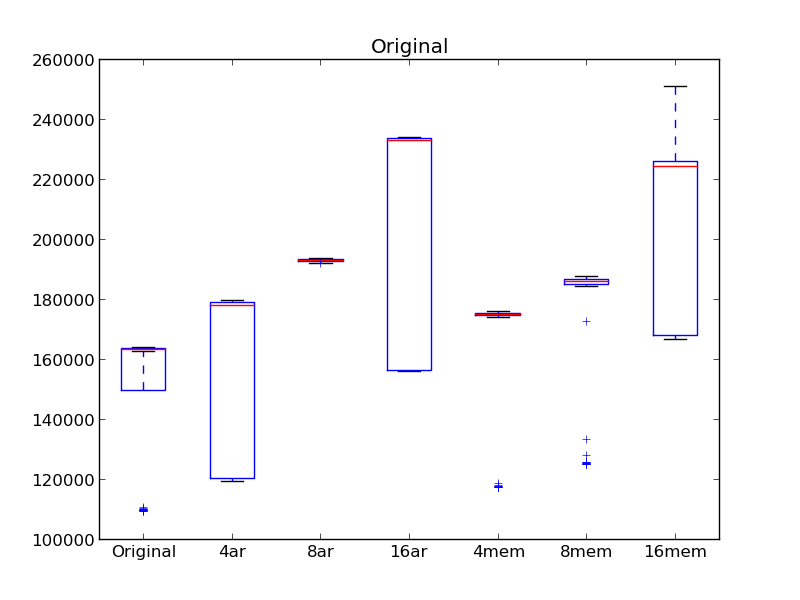
\includegraphics[scale=0.5]{imagenes/arvsmemcropflip.png}
\caption{Cropflip: intensidad de cómputo vs. bus de memoria}
\label{fig:graficos_cropflip2}
\end{figure}

\begin{tabular}{l|r|r} %cropFlip
 & Esperanza & Desvío estándar \\
 original & 150.074 & 18.011 \\
 4 aritméticas & 151.369 & 22.978 \\
 8 aritméticas & 192.910 & 316 \\
 16 aritméticas & 210.302 & 27.340 \\
 4 memoria & 165.522 & 16.591 \\
 8 memoria & 174.043 & 18.584 \\
 16 memoria & 206.404 & 25.225
\end{tabular}

\smallskip

Hallamos que tanto las operaciones aritméticas como los accesos a memoria afectan el tiempo de ejecución de forma similar. %

\subsection{Filtro sierpinski}
En cada iteración de la implementación en assembler del filtro sierpinski se procesan cuatro píxeles. Esto permite manejar cada píxel en un registro, si se toman sus valores de $r$, $g$, $b$ y $\alpha$ como enteros de 4 bytes o como decimales de precisión simple (floats). En cada iteración, se realizan los siguientes pasos: 
\begin{itemize}
\item Se toman 4 píxeles y se desempaquetan en cuatro registros xmm, extendiendo sus valores a 4 bytes.
\item Como $i$ es igual para cada columna, se calcula $\frac{i}{filas}*255$ en un registro de 8 bytes, antes de repetirlo cuatro veces en xmm4.
\item Se repite cuatro veces el valor de $j$ como entero de 4 bytes en xmm5.
\item Se le suma a cada entero de $j$ 0, 1, 2 o 3, de forma que corespondan a las mismas columnas que los píxeles. 

Estado de los registros:

\begin{tabular}{c r|r|r|r} 
& 96 & 64 & 32 & 0 \\
xmm0 & $r(i,j)$ & $g(i,j)$ & $b(i,j)$ & $a(i,j)$ \\
xmm1 & $r(i,j+1)$ & $g(i,j+1)$ & $b(i,j+1)$ & $a(i,j+1)$ \\
xmm2 & $r(i,j+2)$ & $g(i,j+2)$ & $b(i,j+2)$ & $a(i,j+2)$ \\
xmm3 & $r(i,j+3)$ & $g(i,j+3)$ & $b(i,j+3)$ & $a(i,j+3)$ \\
xmm4 & $i$ & $i$ & $i$ & $i$ \\
xmm5 & $j$ & $j+1$ & $j+2$ & $j+3$ \\
\end{tabular}

\item Se multiplica por 255 cada valor de xmm5. Luego se lo convierte a $float$ para dividirlo por la cantidad de columnas, para luego convertirlo de vuelta a entero, truncando.
\item Se ejecuta un xor bit a bit entre xmm4 y xmm5. La división por 255 se posterga para no perder precisión.
\item Se multiplica el valor de $r$, $g$, $b$ y $\alpha$ de cada píxel por el coeficiente correspondiente. Para esto se guarda una copia de xmm4, se repite cuatro veces el valor del coeficiente de la posición del píxel en xmm5 y se efectúa la multiplicación. Luego se realiza la división por 255, convirtiendo a $float$ antes, y truncando después. 
\item Se empaqueta el resultado a bytes y se asigna a los píxeles correspondientes.
\end{itemize}

\subsubsection{Experimentación con optimizaciones}

Al comparar la versión en assembler con la versión en C con las distintas optimizaciones, se obtuvieron estos resultados: (ver Figura ~\ref{fig:graficos_sierpinski})

\begin{figure}[htbp]
\centering
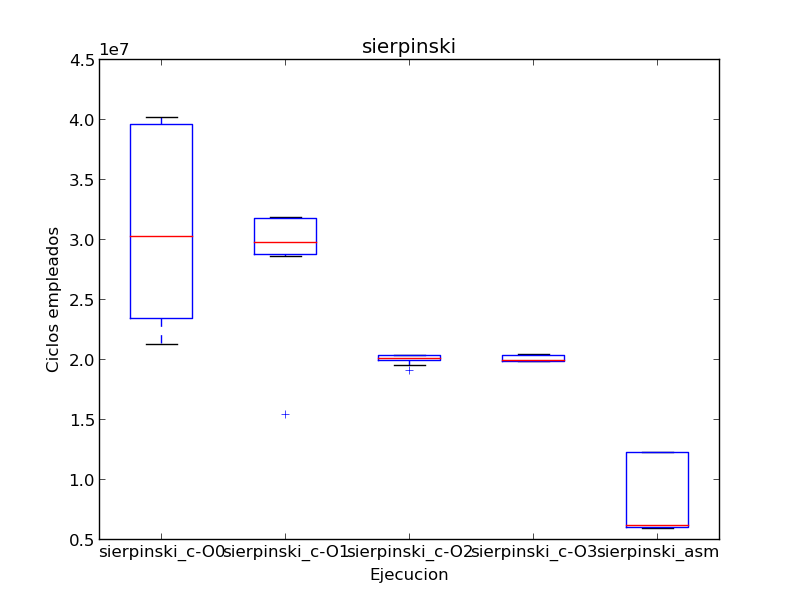
\includegraphics[scale=0.33]{imagenes/tiempossierpinski.png}
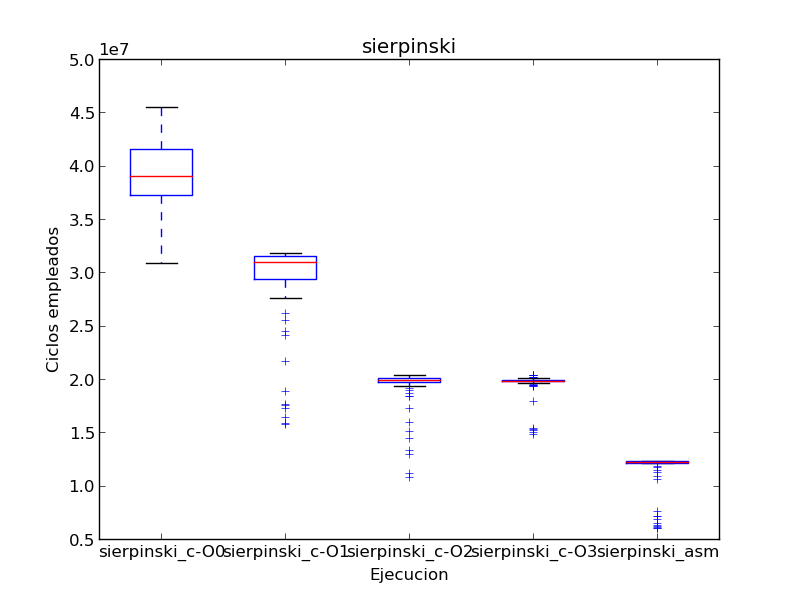
\includegraphics[scale=0.33]{imagenes/tiempossierpinski100.png}
\caption{Sierpinski: 10 mediciones (izquierda) vs. 100 (derecha)}
\label{fig:graficos_sierpinski}
\end{figure}

\begin{tabular}{c|r|r} %sierpinski
 & Esperanza & Desvío estándar \\
 c(-O0) & 38.405.241 & 6.357.934 \\
 c(-O1) & 27.748.695 & 6.024.400 \\
 c(-O2) & 18.288.602 & 3.640.527 \\
 c(-O3) & 18.503.651 & 3.307.329 \\
 asm & 10.894.441 & 2.575.915
\end{tabular}
(valores en ciclos de clock)

\smallskip
Se puede ver que las optimizaciones de C reducen apreciablemente el tiempo de ejecución, aunque \texttt{-O3} es prácticamente igual a \texttt{-O2}. Aun con todas las optimizaciones el tiempo de ejecución en C es alrededor de un 50 $\%$ del tiempo de ejecución en assembler. %[hay que justificarlo?].

\subsubsection{Experimentación bus de memoria vs. tiempo de cómputo}

Estos son los resultados obtenidos al comparar el impacto de las instrucciones aritméticas con el de los accesos a memoria: (ver Figura ~\ref{fig:graficos_sierpinski2})

\begin{figure}[htbp]
\centering
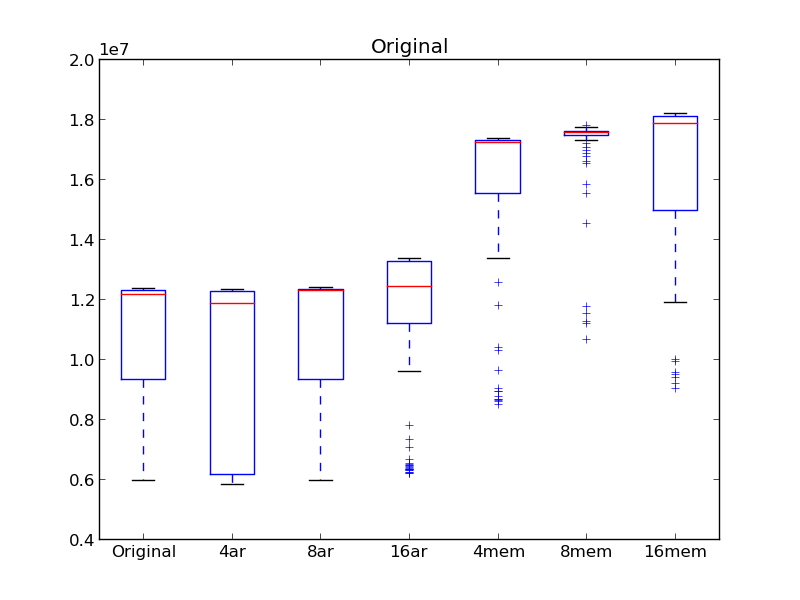
\includegraphics[scale=0.5]{imagenes/arvsmemsierpinski.png}
\caption{Sierpinski: intensidad de cómputo vs. bus de memoria}
\label{fig:graficos_sierpinski2}
\end{figure}

\begin{tabular}{l|r|r} %sierpinski
 & Esperanza & Desvío estándar \\
 original & 11.013.853 & 1.562.466 \\
 4 aritméticas & 10.154.046 & 2.028.326 \\
 8 aritméticas & 11.064.048 & 1.674.657 \\
 16 aritméticas & 11.943.112 & 1.833.049 \\
 4 memoria & 16.168.994 & 1.612.332 \\
 8 memoria & 17.476.791 & 187.870 \\
 16 memoria & 16.939.160 & 1.334.525
\end{tabular}

Hallamos que el principal factor limitante es el bus de memoria. Se puede ver en los gráficos que agregar algunos accesos a memoria afecta apreciablemente el tiempo de ejecución, algo que no ocurre con las operaciones aritméticas. Sin embargo, el impacto de agregar 8 o 16 operaciones con la memoria no es mucho mayor al de agregar 4. Esto pude deberse a que las instrucciones adicionales produjeron $hits$ en la caché, a pesar de que se intentó evitarlo.

\subsection{Filtro bandas}
En este filtro se busca reemplazar cada píxel por un tono X de grises que es elegido a partir de la suma de sus componentes RGB. La suma de los componentes RGB lo llamaremos $B$ y a partir de este $B$ se ingresará a un caso específico que determinará el tono de gris que corresponde al píxel.
En cada iteración de la implementación en assembler del filtro bandas se procesan dos píxeles. Esto permite manejar ambos píxeles en un solo registro durante toda la iteración del ciclo, ya que se busca sumar los valores red, green y blue, que no exceden 765. Como este número se puede expresar como $short$, al tomar los dos píxeles convertiendo cada byte en short se ocupan los 16 bytes del registro xmm. La decisión de trabajar con dos píxeles se tomó por simplicidad, pero esto repercute en que se genera una mayor cantidad de accesos a memoria.
En cada iteración, se realizan los siguientes pasos: 
\begin{itemize}
\item Se toman los dos píxeles correspondientes y se extiende directamente cada byte de cada píxel en shorts, utilizando la instrucción \texttt{pmovzxbw}.
\item Se aplica una mascara para sacar los $\alpha$ de transparencia, ya que no se desea sumar su valor al $B$ que determinará el tono $X$ de grises que corresponde a cada píxel.
\item Se utiliza la función \texttt{phaddw} dos veces para sumar horizontalmente los valores RGB, obteniendo así el $B$ de cada píxel en los dos shorts de la parte baja del registro xmm.
\item Se analiza en que caso entran estos $B$ mediante comparaciones con los valores que corresponde, y si en alguna comparación se encuentra una $B$ que la cumpla, esta se modifica con el tono $X$ de grises que corresponda para ese caso, como se ve en la figura para un caso particular:

\begin{tabular}{r r|r|r|r|r|r|r|r||l} 

& 112 & 96 & 72 & 64 & 48 & 32 & 16 & 0 \\
xmm1 &      &      &      &      &      &      & $B_0$  & $B_1$  &  Supongamos que 288 $\leq B_0$\textless 480 \\ 
xmm4 & 0000 & 0000 & 0000 & 0000 & 0000 & 0000 & FFFF   & 0000   & $B_0 \geq$288 (del ciclo anterior)          \\ 
xmm2 & 480  & 480  & 480  & 480  & 480  & 480  & 480    & 480    &                                             \\
xmm2 & 0000 & 0000 & 0000 & 0000 & 0000 & 0000 & FFFF   & 0000   & pcmpgtw xmm2, xmm1                          \\
xmm2 & 0000 & 0000 & 0000 & 0000 & 0000 & 0000 & FFFF   & 0000   & 288$\leq B\leq$480 (pand)                   \\ 
xmm5 & 192  & 192  & 192  & 192  & 192  & 192  & 192    & 192    & Valor que corresponde                       \\
xmm5 & 0    & 0    & 0    & 0    & 0    & 0    & 192    & 0      & pand con xmm2                               \\
xmm2 & FFFF & FFFF & FFFF & FFFF & FFFF & FFFF & 0000   & FFFF   & Niego los que cumplen                       \\ 
xmm1 &      &      &      &      &      &      & 0      & $B_1$  & Queda igual el que no cumple (pand)         \\ 
xmm1 &      &      &      &      &      &      & 192    & $B_1$  & Se agrega el valor (por)                    \\
\end{tabular}


\item Luego de determinar el tono $X$ para cada píxel (llamemos $X_0$ al tono que corresponde al primer píxel, y $X_1$ al segundo), se utiliza un shuffle para que en la parte alta del registro xmm esté el valor de $X_0$ en los 4 shorts del píxel, y otro shuffle para poner el $X_1$ en la parte baja.
\item Por ultimo se empaqueta el registro pasando de word a byte (esto no afecta el valor de los X ya que estos van de 0 a 255), y se carga la parte baja del registro en la posicion de memoria del cual pertenecen esos dos píxeles.
\end{itemize}

\subsubsection{Experimentación con optimizaciones}

Al comparar la versión en assembler con la versión en C con las distintas optimizaciones, se obtuvieron estos resultados: (ver Figura ~\ref{fig:graficos_bandas})
\begin{figure}[htbp]
\centering
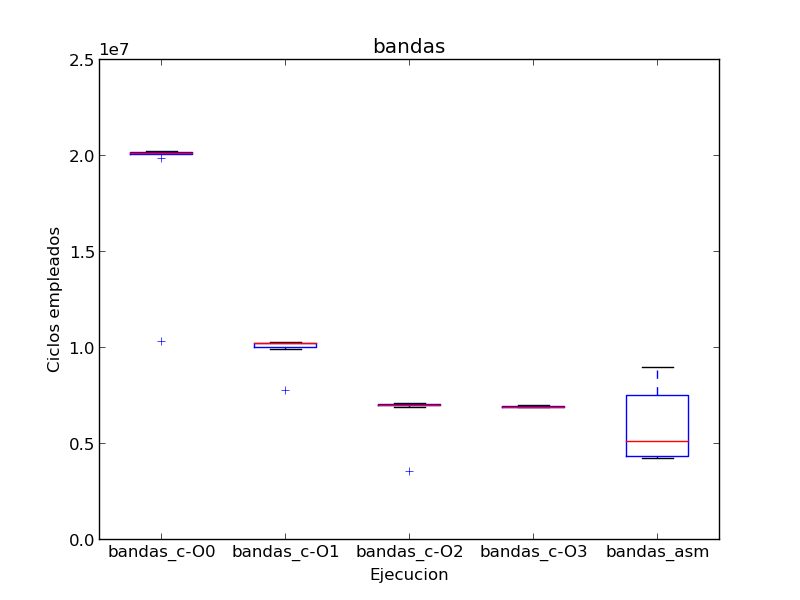
\includegraphics[scale=0.33]{imagenes/tiemposbandas.png}
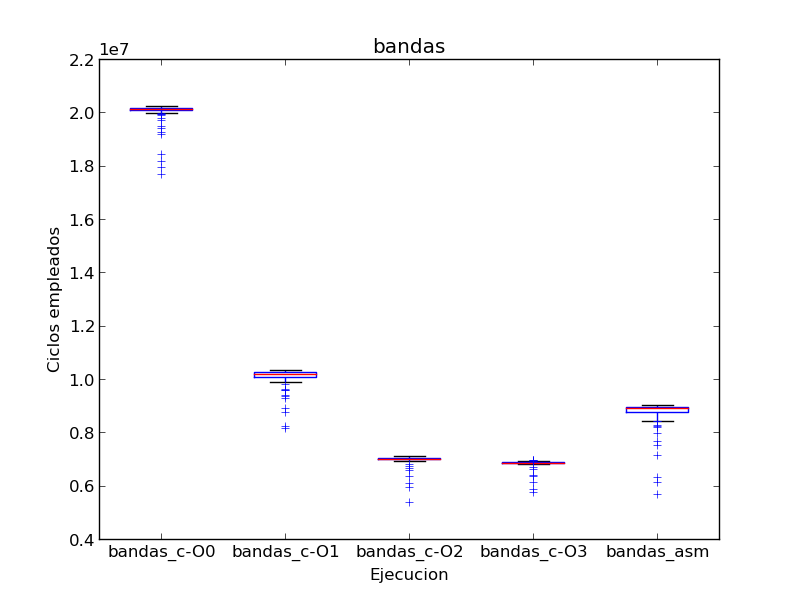
\includegraphics[scale=0.33]{imagenes/tiemposbandas100.png}
\caption{Bandas: 10 mediciones (izquierda) vs. 100 (derecha)}
\label{fig:graficos_bandas}
\end{figure}

\begin{tabular}{c|r|r} %bandas
 & Esperanza & Desvío estándar \\
 c(-O0) & 19.195.427 & 2.375.825 \\
 c(-O1) & 9.528.026 & 1.593.059 \\
 c(-O2) & 6.584.477 & 1.118.761 \\
 c(-O3) & 6.458.837 & 1.086.782 \\
 asm & 8.222.785 & 1.551.852
\end{tabular}
(valores en ciclos de clock)


\smallskip
Se puede ver que las optimizaciones de C reducen apreciablemente el tiempo de ejecución, aunque \texttt{-O3} es prácticamente igual a \texttt{-O2}. El tiempo de ejecución en ASM es mayor a las versiones \texttt{-O2} y \texttt{-O3}. Esto se debe a que solo procesamos de a dos píxeles.

\subsubsection{Experimento de saltos Condicionales}

Al eliminar los saltos condicionales, observamos que el tiempo de cómputo con \texttt{-O1} se redujo considerablemente, como se puede ver en la imagen:

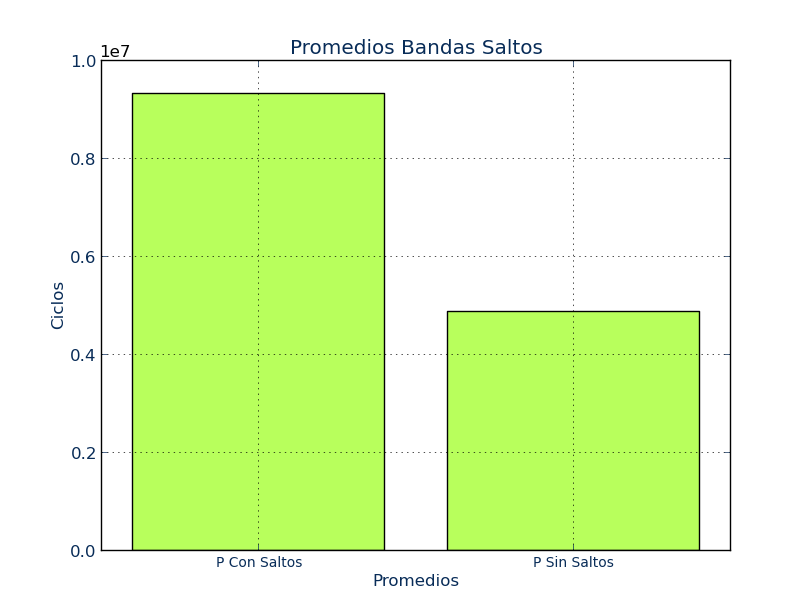
\includegraphics[scale=0.5]{imagenes/PromedioSaltos.png}

Se pude obsevar que al sacar cuatro casos condicionales, la cantidad de ciclos se redujo en promedio aproximadamente a la mitad. Suponemos que esto se debe en primer lugar a que solo se entra en un caso para determinar el tono de gris; la reducción de ciclos puede provenir tambien del $pipeline$, ya que al haber un solo caso del $if$, el $pipeline$ puede recuperar rapidamente su ritmo y seguir con la ejecución de los ciclos en paralelo.

\subsection{Filtro motion blur}
En el filtro motion blur, cada píxel es afectado por sí mismo y cuatro de sus vecinos, en diagonal. Por lo tanto, para el procesamiento de cada píxel son necesarios 5. Procesamos de a 4 píxeles de la siguiente forma:
\begin{itemize}
\item Se ubica el dato de en la matriz src y se toman los 5 conjuntos de píxeles de la diagonal que se va a procesar, cada uno en un registro xmm.
\item Se desempaqueta cada uno en dos registros, de modo que cada píxel ocupe una quadword.
\item Se efectua la suma entre todos los píxeles de una misma diagonal antes de la division por 5 para poder hacer división entera sin perder precisión.
\item Para optimizar la división por una constante, se aprovecha el hecho de que el dividendo está acotado por 255*5=1275, y que $(\forall\ 0 \leq n \leq 1275), \frac{n}{5}=\frac{n*3277}{2^{14}} $ %justificar mas esto? nah
para reemplazar la división por una multiplicación y una división por una potencia de 2, que se traduce en un $shift\ left$, que son operaciones considerablemente menos costosas para el procesador. Es necesario desempaquetar una vez más para que las operaciones no produzcan overflow.
\item Llegado este punto, ya se obtuvieron los valores finales de las componentes de cada píxel, se empaqueta todo nuevamente y se guarda en la matriz destino.
\end{itemize}
Este proceso sirve para calcular los valores de los píxeles a distancia mayor a 2 de los bordes, a los que no cumplen esto se los pinta de color negro. Para esto, resulta más simple realizar un ciclo separado que recorra exclusivamente los bordes, asignándoles el valor 0.

\subsubsection{Experimentación con optimizaciones}

Al comparar la versión en assembler con la versión en C con las distintas optimizaciones, se obtuvieron estos resultados: (ver Figura ~\ref{fig:graficos_mblur})

\begin{figure}[htbp]
\centering
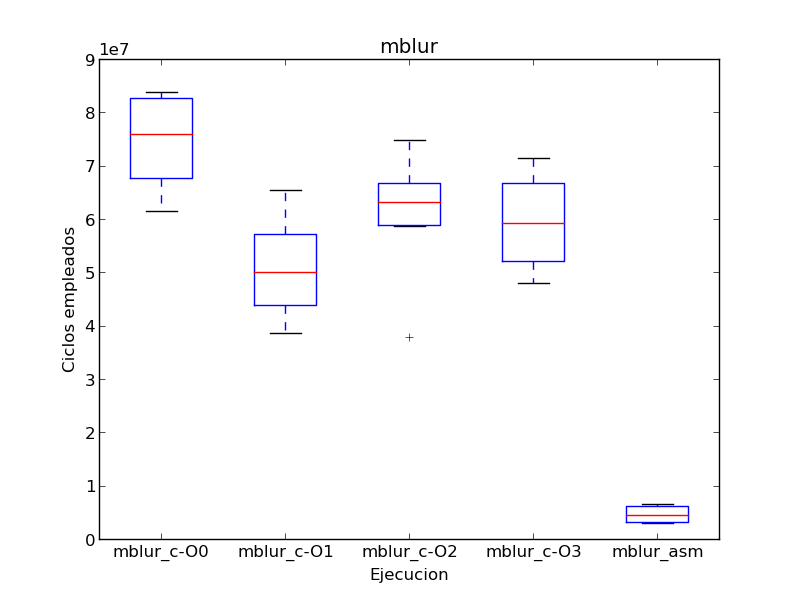
\includegraphics[scale=0.33]{imagenes/tiemposmblur.png}
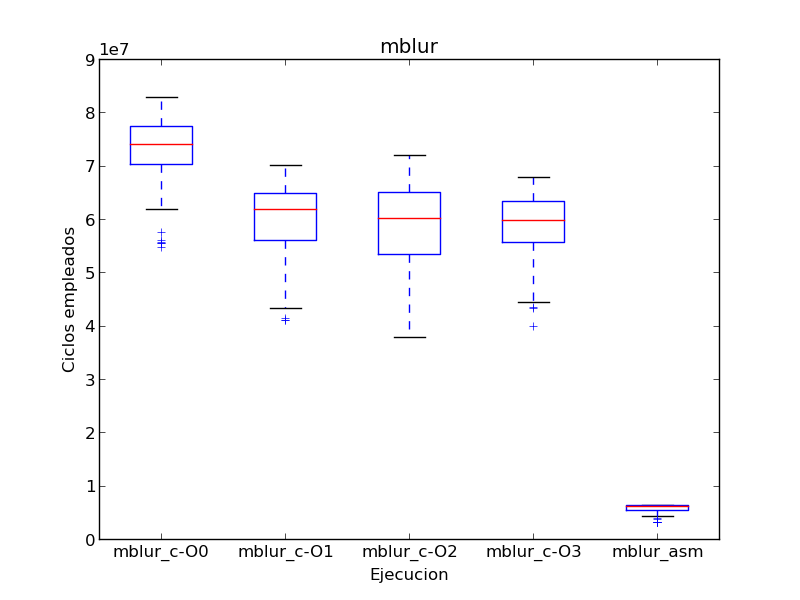
\includegraphics[scale=0.33]{imagenes/tiemposmblur100.png}
\caption{Motion blur: 10 mediciones (izquierda) vs. 100 (derecha)}
\label{fig:graficos_mblur}
\end{figure}

\begin{tabular}{c|r|r} %mblur
 & Esperanza & Desvío estándar \\
 c(-O0) & 71.583.675 & 10.967.397 \\
 c(-O1) & 58.938.095 & 10.777.338 \\
 c(-O2) & 57.580.907 & 12.153.264 \\
 c(-O3) & 57.209.805 & 10.382.008 \\
 asm & 5.499.959 & 1.281.279
\end{tabular}
(valores en ciclos de clock)

\smallskip
Se puede ver que las optimizaciones de C no reducen apreciablemente el tiempo de ejecución. \texttt{-O2} y \texttt{-O3} tardan más que \texttt{-O1}. El tiempo de ejecución en C es alrededor de diez veces el tiempo de ejecución en assembler.


\section{Conclusiones}

Comparando los resultados de performance de las versiones ASM y C en cada filtro, se puede concluir que el ASM siempre es más eficiente que la versión no optimizada de C. En cuanto a las optimizaciones, reducen considerablemente el tiempo de ejecución del código C. La optimización \texttt{-O3}, que es la que aplica vectorización de ciclos, sólo marca una diferencia en el filtro cropflip, mientras que en los otros casos no modifica el tiempo de ejecución. Analizando el resultado del $objdump$, se puede concluir que ésto se debe a que es el único caso en el que el compilador utiliza operaciones SIMD, procesando de ésta forma 4 píxeles simultáneamente. Presumiblemente, en los otros filtros no hace uso del SIMD porque la complejidad de los ciclos se lo impide, y se ve limitado a procesar un píxel por ciclo, deteriorando la performance.

Al comparar el impacto de las operaciones aritméticas con el de los accesos a memoria se esperaba obtener una mayor influencia de los accesos a memoria. Esto es porque un acceso a memoria involucra, como mínimo, las siguientes microoperaciones:
\begin{itemize}
\item Obtener la dirección a leer (esto ya son varios pasos, puede ser una operación aritmética en sí).
\item Escribir la dirección en el bus de memoria.
\item Realizar el acceso a memoria. Si la dirección se encuentra almacenada en memoria caché, ésto se puede realizar con relativa rapidez, de lo contrario obtener los datos de la memoria RAM consume una cantidad considerablemente mayor de tiempo.
\item Mover el resultado al registro indicado.
\end{itemize}
En cambio, una operación aritmética, incluso una división, se reduce a un algoritmo a ser ejecutado por una ALU. 

Sin embargo, esto se vio reflejado solamente en el filtro sierpinski. En el cropflip, el impacto de operaciones aritméticas y accesos a memoria fue muy similar. Ésto puede deberse a que el filtro sierpinski tiene una gran cantidad de operaciones aritméticas en relación con la cantidad de accesos a memoria, por lo que añadir éstos últimos produce un mayor impacto, mientras que cropflip efectúa principalmente accesos a memoria, lo que ocasiona que el añadido de operaciones aritméticas sea casi tan influyente como seguir añadiendo accesos.

Las optimizaciones reducen los accesos a memoria. Por lo explicado en el párrafo anterior, esto garantiza una mayor velocidad. Los flags \texttt{-O1} y \texttt{-O2} reducen, además la cantidad de operaciones aritméticas. \texttt{-O3} genera un código considerablemente más largo que el original, por lo que se espera que los mejores resultados de velocidad se obtengan eliminando la mayor cantidad posible de accesos a memoria y reemplazándolos si es necesario con una cantidad limitada de operaciones aritméticas.

En resumen, el modo de programación SIMD es muy conveniente en términos de velocidad, ya que si se explotan sus posibilidades se puede reducir el tiempo de cómputo a una fracción del tiempo de ejecución en C, incluso optimizado. Sin embargo, la programación assembler es más compleja ya que este lenguaje tiene una relación línea a línea con el código máquina. El lenguaje C, en cambio, está más cerca del lenguaje humano: el ASM permite una interacción más directa con los registros, mientras que el C provee una capa de abstracción. Sin embargo, hay una relación directa entre el código C y el ASM, lo que no se puede decir de lenguajes de más alto nivel, como C++.

\newpage 
\section{Enunciado}
\subsection{Filtro cropflip}

Programar el filtro \textit{cropflip} en lenguaje C y luego en ASM haciendo 
uso de las instrucciones vectoriales (\textbf{SSE}).

% ******************************************************************************
\vspace*{0.3cm} \noindent
\textbf{Experimento 1.1 - análisis el código generado}

En este experimento vamos a utilizar la herramienta \verb|objdump| para 
verificar como el compilador de C deja ensamblado el código C.

Ejecutar 
\begin{codesnippet}
\begin{verbatim}
objdump -Mintel -D cropflip_c.o
\end{verbatim}
\end{codesnippet}

¿Cómo es el código generado? 
Indicar
\begin{inparaenum}[\itshape a\upshape)]
    \item Por qué cree que hay otras funciones además de \verb|cropflip_c|
    \item Cómo se manipulan las variables locales
    \item Si le parece que ese código generado podría optimizarse
\end{inparaenum}

% ******************************************************************************
%\newpage
\vspace*{0.3cm} \noindent
\textbf{Experimento 1.2 - optimizaciones del compilador}

Compile el código de C con flags de optimización. Por ejemplo, pasando el flag 
\verb|-O1|\footnote{agregando este flag a \texttt{CCFLAGS64} en el makefile}. 
Indicar
\begin{inparaenum}
    \item Qué optimizaciones observa que realizó el compilador
    \item Qué otros flags de optimización brinda el compilador
    \item Los nombres de tres optimizaciones que realizan los compiladores.
\end{inparaenum}

% ------------------------------------------------------------------------------
% ------------------------------------------------------------------------------

\subsection{Mediciones}

Realizar una medición de performance \emph{rigurosa} es más difícil de lo 
que parece. 
En este experimento deberá realizar distintas mediciones de performance 
para verificar que sean buenas mediciones.

En un sistema ``ideal'' el proceso medido corre solo, sin ninguna 
interferencia de agentes externos. 
Sin embargo, una PC no es un sistema ideal. 
Nuestro proceso corre junto con decenas de otros, tanto de usuarios como 
del sistema operativo que compiten por el uso de la CPU. 
Esto implica que al realizar mediciones aparezcan ``ruidos'' o 
``interferencias'' que distorsionen los resultados.

El primer paso para tener una idea de si la medición es buena o no, 
es tomar varias muestras. 
Es decir, repetir la misma medición varias veces.
Luego de eso, es conveniente descartar los outliers
\footnote{en español, valor atípico: \url{http://es.wikipedia.org/wiki/Valor_atípico}}, 
que son los valores que más se alejan del promedio. 
Con los valores de las mediciones resultantes se puede calcular el promedio 
y también la varianza, que es algo similar el promedio de las distancias al 
promedio\footnote{en realidad, elevadas al cuadrado en vez de tomar el módulo}.

Las fórmulas para calcular el promedio $\mu$ y la varianza $\sigma^2$ son

$$
\mu = \frac{1}{n}\sum_{i=1}^{n} x_i \qquad \sigma^2 = \frac{\displaystyle\sum_{i=1}^{n}(x_i - \mu)^2} {n}
$$

% ******************************************************************************
\newpage
\vspace*{0.3cm} \noindent
\textbf{Experimento 1.3 - calidad de las mediciones}

\begin{enumerate}
    \item Medir el tiempo de ejecución de cropflip 10 veces. 
    \item Implementar un programa en C que no haga más que ciclar 
            infinitamente sumando 1 a una variable. 
            Lanzar este programa tantas veces como \emph{cores lógicos} tenga 
            su procesador. 
            Medir otras 10 veces mientras estos programas corren de fondo.
    \item Calcular el promedio y la varianza en ambos casos.
    \item Consideraremos outliers a los 2 mayores tiempos
     de ejecución de la medicion a) y también a los 2 menores,
     por lo que los descartaremos. Recalcular el promedio y la varianza después de hacer este descarte.
    \item Realizar un gráfico que presente estos dos últimos items.
\end{enumerate}

A partir de aquí todos los experimentos de mediciones deberán hacerse igual 
que en el presente ejercicio: tomando 10 mediciones, luego descartando 
outliers y finalmente calculando promedio y varianza.

% ******************************************************************************
%\newpage
\noindent\textbf{Experimento 1.4 - secuencial vs. vectorial}

En este experimento deberá realizar una medición de las diferencias de 
performance entre las versiones de C y ASM (el primero con -O0, -O1, -O2 y -O3) 
y graficar los resultados.

% ******************************************************************************
\vspace*{0.3cm} \noindent
\textbf{Experimento 1.5 - cpu vs. bus de memoria}

Se desea conocer cual es el mayor limitante a la
performance de este filtro en su versión ASM.

¿Cuál es el factor que limita la performance en este caso?
En caso de que el limitante fuera la intensidad de cómputo, entonces 
podrían agregarse instrucciones que realicen accesos a memoria extra y la
performance casi no debería sufrir. 
La inversa puede aplicarse, si el limitante es la cantidad de accesos a memoria.
\footnote{también podría pasar que estén más bien balanceados y que agregar
cualquier tipo de instrucción afecte sensiblemente la performance}
	
Realizar un experimento, agregando 4, 8 y 16 instrucciones aritméticas 
(por ej \verb|add rax, rbx|) analizando como varía el tiempo de ejecución.
Hacer lo mismo ahora con instrucciones de acceso a memoria, haciendo 
mitad lecturas y mitad escrituras (por ejemplo, agregando dos 
\verb|mov rax, [rsp]| y dos \verb|mov [rsp+8], rax|).\footnote{Notar que en el caso de acceder a \texttt{[rbp]} o \texttt{[rsp+8]} probablemente haya siempre hits en la cache, por lo que la medición no será de buena calidad. Si se le ocurre la manera, realizar accesos a otras direcciones alternativas.}
	
Realizar un único gráfico que compare:
\begin{inparaenum}
    \item La versión original
    \item Las versiones con más instrucciones aritméticas
    \item Las versiones com más accesos a memoria
\end{inparaenum}

Acompañar al gráfico con una tabla que indique los valores graficados.  
  
%\vspace*{0.3cm} \noindent
%\textbf{Experimento 1.6 (\textit{opcional}) - secuencial vs. vectorial (parte II)}
%
%
%Si vemos a los pixeles como una tira muy larga de
%bytes, este filtro en realidad no requiere \emph{casi}
%ningún procesamiento de datos en paralelo. Esto podría
%significar que la velocidad del filtro de C puede
%aumentarse hasta casi alcanzar la del de ASM. ¿ocurre esto?
%	
%Modificar el filtro para que en vez de acceder
%a los bytes de a uno a la vez se accedan como
%tiras de 64 bits y analizar la performance.

% ------------------------------------------------------------------------------
% ------------------------------------------------------------------------------

\subsection*{Filtro \textit{Sierpinski}}

Programar el filtro \textit{Sierpinski} en lenguaje C y en en ASM haciendo 
uso de las instrucciones vectoriales (\textbf{SSE}).

% ******************************************************************************
\vspace*{0.3cm} \noindent
\textbf{Experimento 2.1 - secuencial vs. vectorial}

Analizar cuales son las diferencias de performace entre las versiones de C 
y ASM de este filtro, de igual modo que para el experimento 1.4.

% ******************************************************************************
\vspace*{0.3cm} \noindent
\textbf{Experimento 2.1 - cpu vs. bus de memoria}

¿Cuál es el factor que limita la performance en este filtro?
Repetir el experimento 1.5 para este filtro.

\subsection*{Filtro \textit{Bandas}}

Programar el filtro \textit{Bandas} en lenguaje C y en en ASM haciendo uso de 
las instrucciones vectoriales (\textbf{SSE}).

% ******************************************************************************
\vspace*{0.3cm} \noindent
\textbf{Experimento 3.1 - saltos condicionales}

Se desea conocer que tanto impactan los saltos condicionales en el código 
de filtro Bandas con \verb|-O1| (la versión en C).\\
Para poder medir esto de manera aproximada, remover el código
que detecta a que banda pertenece cada pixel, dejando
sólo una banda.
Por más que la imagen resultante no sea correcta, será posible tomar una
medida aproximada del impacto de los saltos condicionales.
Analizar como varía la performance. 

% ******************************************************************************
\vspace*{0.3cm} \noindent
\textbf{Experimento 3.2 - secuencial vs. vectorial}

Repetir el experimento 1.4 para este filtro.

% ------------------------------------------------------------------------------
% ------------------------------------------------------------------------------

\subsection*{Filtro \textit{Motion Blur}}
Programar el filtro \textit{mblur} en lenguaje C y en ASM haciendo uso de 
las instrucciones \textbf{SSE}.

% ******************************************************************************
\vspace*{0.3cm} \noindent
\textbf{Experimento 4.1}

Repetir el experimento 1.4 para este filtro


\section{Bibliografía}
\begin{itemize}
\item Apuntes de clase
\item Manuales de Intel
\item https://gcc.gnu.org/onlinedocs/gcc/Optimize-Options.html
\end{itemize}


\end{document}
